\documentclass[10pt]{beamer}

\usetheme[progressbar=frametitle]{metropolis}

\usepackage{booktabs}
\usepackage[scale=2]{ccicons}

\usepackage{minted}
\newminted{haskell}{tabsize=4}
\usemintedstyle{trac}

\usepackage{pgf}
\usepackage{tikz}
\usetikzlibrary{arrows,automata}

\usepackage{amsmath}

\usepackage{pgfplots}
\usepgfplotslibrary{dateplot}

\usepackage{xspace}
\newcommand{\themename}{\textbf{\textsc{metropolis}}\xspace}

\title{Ragax: Ragalur Expressions}
\subtitle{Using derivatives to validate Indian Classical Music}
\date{2 May 2018}
\author{Walter Schulze}
\institute{Amsterdam Functional Programming Meetup}

\usepackage{xcolor}
\def\valid{${\color{mLightGreen} \checkmark}$}
\def\invalid{{\color{mLightBrown} x}}

\begin{document}

\maketitle

\begin{frame}{Key Takeaways}

\note{
Hello

Welcome to my talk on Ragax or Ragalur Expressions ... pun intended.

I am going to use derivatives to show you how easy it is to implement your own regular expression matcher function.
Derivatives are so trivial and extendable, that you should also be able to invent your own operators.
This also means that we can extend it to Context Free Grammars, which we can use for Ragas, the whole point of this talk.

Ok, lets go.
}

\begin{itemize}
\item implement matcher
\item invent operators
\item \textbf{derivatives are intuitive and extendable}
\item generate music
\end{itemize}

\end{frame}

\begin{frame}[fragile]{Regular Expressions}

\note{
Lets just do a quick review of regular expressions to make sure we are on the same page.
Here we see an expression that matches a string that starts with an 'a',
which is followed by any number of 'a's and 'b's

We can also write it like this (point to bottom).
Which is the syntax we'll use in the rest of this talk.
So the concat operator is represented with a dot.

Also notice that we are not doing substring matching and that we only match the whole string.
See for example "ba" that is not matched.

Any questions?
}

$$
a(a|b)*
$$
\begin{center}
\begin{tabular}{ll}
ab & \valid \\
aabbba & \valid \\
ac & \invalid \\
ba & \invalid \\
\end{tabular}
\end{center}
$$
a \cdot (a\ |\ b)^{*}
$$
\end{frame}

\begin{frame}{What is a Brzozowski Derivative}

\note{
What is a derivative? ... The derivative of an expression is the expression that is left to match after the given character has been matched.
So the derivative of the expression a, a or b star with respect to a is a or b star.

Here are some more examples:

\begin{itemize}
\item The derivative of abc with respect to a is ab.
\item With an "or" we have to try both alternatives so we take the derivative of both.
\item The derivative of c with respect to c is the empty string
\item The derivative of a star with respect to a stays a star.
\end{itemize}

I will now explain the formal rules, but I hope that these examples give you an intuition.
}

The derivative of an expression is the expression that is left to match after the given character has been matched
\cite{brzozowski1964derivatives}.

\begin{center}
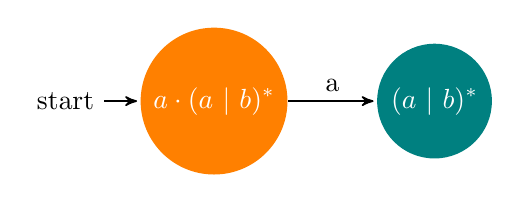
\begin{tikzpicture}[->,>=stealth',shorten >=1pt,auto,node distance=2.8cm,semithick]
    \tikzstyle{every state}=[fill=orange,draw=none,text=white]

    \node[initial,state]       (A)              {$a \cdot (a\ |\ b)^{*}$};
    \node[state,fill=teal]     (B) [right of=A] {$(a\ |\ b)^{*}$};

    \path (A) edge              node {a} (B);
\end{tikzpicture}
\end{center}

\begin{center}
\begin{tabular}{lll}
$\partial_a a \cdot b \cdot c$ & = & $b \cdot c$ \\
$\partial_a (a \cdot b\ |\ a \cdot c)$ & = & $(b\ |\ c)$ \\
$\partial_c c$ & = & $\epsilon$ \\
$\partial_a a^{*}$ & = & $a^{*}$ \\
\end{tabular}
\end{center}

\end{frame}

\begin{frame}{Basic Operators}

\note{
First we have a few basic operators.

If we think of the set of strings that matches a regular expression, then the empty set does not match any strings.

The empty string matches only the empty string.

The character a matches only the character a, not the substring a, remember we are only dealing with whole strings.

And then we have the rest: concat, zero or more and or.
}

\begin{center}
\begin{tabular}{l|r}
empty set & $\emptyset$ \\
empty string & $\varepsilon$ \\
character & $a$ \\
concatenation & $r \cdot s$ \\
zero or more & $r^*$ \\
logical or & $r\ |\ s$ \\
\end{tabular}
\end{center}
\end{frame}

\begin{frame}[fragile]

\note{
We can represent this in haskell using an algebriac data type.

But you don't need to understand the haskell to understand most of this talk.

I just thought that for those who know it, it might make the math easier.
}

\frametitle{Basic Operators}
\begin{center}
\begin{minted}{haskell}
data Regex = EmptySet
  | EmptyString
  | Character Char
  | Concat Regex Regex
  | ZeroOrMore Regex
  | Or Regex Regex
\end{minted}
\end{center}
\end{frame}

\begin{frame}[fragile]{Nullable}

\note{
Before we can explain the derivative algorithm we first need to understand the nullable function.

The nullable function returns true if the set of strings that the regular expression matches includes the empty string.

The emptyset matches no strings, so it also does not match the empty string.

the empty string, well uhm yes

the character a, no, because it only matches the character a

The concatenation of r and s, well only if r and s contain the empty string.

r star, zero or more, includes zero, which is the empty string

r or s, well r or s needs to include the empty string.
}

Does the expression match the empty string.
\begin{center}
\begin{tabular}{l c l}
$\nu(\emptyset)$ & = & false\\
$\nu(\varepsilon)$ & = & true\\
$\nu(a)$ & = & false\\
$\nu(r \cdot s)$ & = & $\nu(r)\ and\ \nu(s)$ \\
$\nu(r^{*})$ & = & true \\
$\nu(r\ |\ s)$ & = & $\nu(r)\ or\ \nu(s)$ \\
\end{tabular}
\end{center}
\end{frame}

\begin{frame}[fragile]{Nullable}

\note{Or if you prefer the haskell}

Does the expression match the empty string.
\begin{center}
\begin{minted}{haskell}
nullable :: Regex -> Bool
nullable EmptySet = False
nullable EmptyString = True
nullable Character{} = False
nullable (Concat a b) = nullable a && nullable b
nullable ZeroOrMore{} = True
nullable (Or a b) = nullable a || nullable b
\end{minted}
\end{center}
\end{frame}

\begin{frame}{Nullable Examples}

\note{
Lets look at some examples or 
maybe you can tell me if there is an example here that you disagree with or don't understand ...
everyone happy?
}

\begin{center}
\begin{tabular}{l c l}
$\nu(a \cdot b \cdot c)$ & = & $\invalid$ \\
$\nu(\varepsilon)$ & = & $\valid$ \\
$\nu(a\ |\ b)$ & = & $\invalid$\\
$\nu(\varepsilon\ |\ a)$ & = & $\valid$\\
$\nu(a \cdot \varepsilon)$ & = & $\invalid$ \\
$\nu((a \cdot b)^{*})$ & = & $\valid$ \\
$\nu(c \cdot (a \cdot b)^{*})$ & = & $\invalid$ \\
\end{tabular}
\end{center}
\end{frame}

\begin{frame}{Derivative Rules}

\note{
Now lets do the formal derivative rules.
The derivative of the emptyset is always going to be the emptyset.
The derivative of the empty string is also always the emptyset.
The empty string does not expect any more characters.  It is done.

The derivative of a single character given the same character is the empty string, 
but otherwise it won't match any string, so it is the emptyset.

The derivative of a concatenation has two cases.
If the left expression is not nullable then we simply take the derivative of the left expression concatenated to the right.
But if the left expression is nullable, then we have to consider the case where we skip over it and take the derivative of the right expression.

The derivative of the zero or more expression is the concatenation of the derivative of the contained expression and the original zero or more expression.
The or expression simply pushes its problems down to its children.
}

\begin{center}
\begin{tabular}{l c l r}
$\partial_a \emptyset$ & = & $\emptyset$ \\
$\partial_a \epsilon$ & = & $\emptyset$ \\
$\partial_a a$ & = & $\epsilon$ \\
$\partial_a b$ & = & $\emptyset \ \ $ for $b \ne a$ \\
$\partial_a (r \cdot s) $ & = & $\partial_a r \cdot s\ $ & $not(\nu(r))$ \\
$\partial_a (r \cdot s) $ & = & $\partial_a r \cdot s\ |\ \partial_a s $ & $\nu(r)$ \\
$\partial_a (r^{*}) $ & = & $\partial_a r \cdot r^{*} $ \\
$\partial_a (r\ |\ s) $ & = & $\partial_a r\ |\ \partial_a s $ \\
\end{tabular}
\end{center}

\end{frame}

\begin{frame}[fragile]{Derivative Rules}

\note{Maybe the haskell is easier to understand.}

\begin{center}
\begin{haskellcode}
deriv :: Regex -> Char -> Regex
deriv EmptyString _ = EmptySet
deriv EmptySet _ = EmptySet
deriv (Character a) c = if a == c 
  then EmptyString else EmptySet
deriv (Concat r s) c =
  let left = deriv r c
      right = deriv s c
  in if nullable r
     then Or (Concat left s) right
     else Concat left s
deriv (ZeroOrMore r) c =
  Concat (deriv r c) (ZeroOrMore r)
deriv (Or r s) c =
  Or (deriv r c) (deriv s c)
\end{haskellcode}
\end{center}
\end{frame}

\begin{frame}[fragile]{Our regular expression matcher}

\note{
Now lets put our two functions together to create a regular expression matcher.

We simply apply the derivative function to each character in the string starting with our regular expression.

If the regular expression that we end up with matches the empty string, then the regular expression matches the input string.
}

$$
\nu(foldl(\partial, r, str))
$$
\begin{center}
\begin{haskellcode}
match :: Regex -> String -> Bool
match expr string = nullable (foldl deriv expr string)
\end{haskellcode}
\end{center}
\begin{center}
\begin{minted}{go}
func matches(r *expr, str string) bool {
    for _, c := range str {
        r = deriv(r, c)
    }
    return nullable(r)
}
\end{minted}
\end{center}
\end{frame}

\begin{frame}[fragile]{Simplification}

\note{
Finally we have simplification which is optional, 
but is great for optimization and will make our examples much more readable.
Here are some of the rules, which should be intuitive:

\begin{itemize}
\item Any expression concatenated with the emptyset is equivalent to the emptyset.
\item Any expression concatenated with the empty string is equivalent to the expression.
\item Any expression ored with itself is equivalent to that expression.
\item Any expression ored with the emptyset is equivalent to that expression.
\item Zero or more, zero or more times, is still just zero or more.
\end{itemize}

Simplification can be part of the derivative function or happen in the constructors.
}

\begin{center}
\begin{tabular}{lll}
$\emptyset \cdot r$ & $\approx$ & $\emptyset$ \\
$r \cdot \emptyset$ & $\approx$ & $\emptyset$ \\
$\varepsilon \cdot r$ & $\approx$ & $r$ \\
$r \cdot \varepsilon$ & $\approx$ & $r$ \\
\\
$r\ |\ r$ & $\approx$ & $r$ \\
$\emptyset\ |\ r$ & $\approx$ & $r$ \\
\\
$(r^{*})^{*}$ & $\approx$ & $r^{*}$ \\
$\varepsilon^{*}$ & $\approx$ & $\varepsilon$ \\
$\emptyset^{*}$ & $\approx$ & $\varepsilon$ \\
\end{tabular}
\end{center}
\end{frame}

\begin{frame}[fragile]{Example: Matching a sequence of notes}

\note{
Ok finally we have another example.
Lets say our characters are musical notes.
And we have an expression for a c major pentatonic scale.

We can take the derivative of the regular expression with respective to each input note to get a resulting regular expression.
It matches if the resulting regular expression is nullable.

Lets walk through it.
The derivative of the initial expression with respect to c is the empty string concatenated with the zero or more expression.
We could simplify that, but lets first try taking the next derivative, for the sake of example.

So the derivative of the empty string concatenated with the zero or more expression is the emptyset concatenated with the zero or more expression, 
but since the empty string is nullabe we also have to take the derivative of the right expression as an alternative.

more notes on next slide...
}

Using a regex we can validate the C Major Pentatonic Scale.
$$
c\cdot(c|d|e|g|a)^{*}
$$
\begin{center}
\begin{tabular}{ll}
ceg & \valid \\
\end{tabular}
\end{center}

\begin{center}
\begin{tabular}{llr}
$\partial_c c\cdot(c|d|e|g|a)^{*}$ & = & $\varepsilon \cdot (c|d|e|g|a)^{*}$\\
$\partial_e \varepsilon \cdot (c|d|e|g|a)^{*}$ & = & 
$(\emptyset \cdot (c|d|e|g|a)^{*})\ |\ (\emptyset | \emptyset | \varepsilon | \emptyset | \emptyset) \cdot (c|d|e|g|a)^{*}$ \\
& = & $(c|d|e|g|a)^{*}$\\
$\partial_g (c|d|e|g|a)^{*}$ & = & $(\emptyset | \emptyset | \emptyset | \varepsilon | \emptyset) \cdot (c|d|e|g|a)^{*}$\\
& = & $(c|d|e|g|a)^{*}$\\
\end{tabular}
\end{center}
\begin{center}
$\nu((c|d|e|g|a)^{*})$ = \valid
\end{center}
\end{frame}

\plain{Questions?}

\note{
Here we can see that every musical note has become the emptyset, except the matching character which has become the empty string.
This big Or is then concatenated with the original zero or more expression.
So here we had to apply the concat rule, the empty string rule, zero or more rule and the or rule.
This easily simplifies to the zero or more expression.

Finally we take the derivative with respect to g which is almost a repeat of the previous equation.

Then we are left with the zero or more expression, which is nullable and means that our string matches the expression and thats it.

This is the part of the talk that everything builds on.
If you don't understand something lets quickly take some time to try and get it right.
At this point you should be able to write your own regular expression matcher function.
}

\begin{frame}[fragile]{Deterministic Finite Automata}

\note{
Lets just take a quick tangent.

Do you remember deterministic finite automata.

Here is one for the regular expression we just evaluated.

Given a c we go the accepting state.
Then we accept any note in the pentatonic scale zero or more times.
Otherwise the song is rejected.
}

$$
c\cdot(c|d|e|g|a)^{*}
$$
\begin{center}
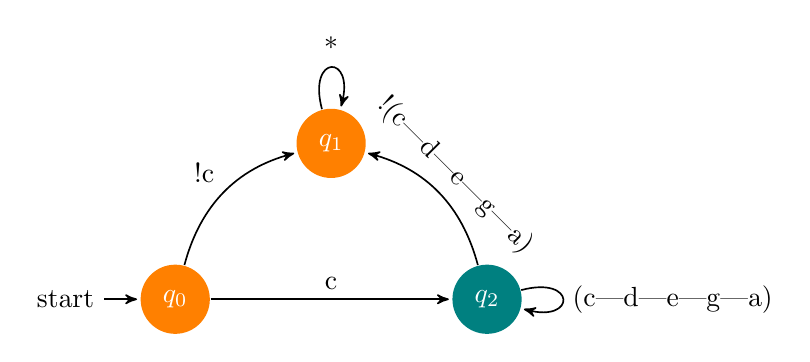
\begin{tikzpicture}[->,>=stealth',shorten >=1pt,auto,node distance=2.8cm,semithick]
  \tikzstyle{every state}=[fill=orange,draw=none,text=white]

  \node[initial,state] (A)                    {$q_0$};
  \node[state]         (B) [above right of=A] {$q_1$};
  \node[state,fill=teal]         (C) [below right of=B] {$q_2$};

  \path (A) edge [bend left]  node {!c} (B)
            edge              node {c} (C)
        (B) edge [loop above] node {*} (B)
        (C) edge [bend right] node [sloped, above] {!(c|d|e|g|a)} (B)
        (C) edge [loop right] node {(c|d|e|g|a)}  (C);
\end{tikzpicture}
\end{center}
\end{frame}

\begin{frame}[fragile]{Memoization and Simplification}

\note{
We can create the same DFA with derivatives by simply memoizing the derivative function for all possible inputs.

The memoized derivative function is the transition function where the regular expressions themselves are states.
The memoized nullable function is the accept function.
Our simplification rules can be used for minimization.

I just think this is so cool that we get this for free.
}

\begin{center}
\begin{tabular}{lll}
$q_0$ & = & $c\cdot(c|d|e|g|a)^{*}$ \\
$q_1$ & = & $\emptyset$ \\
$q_2$ & = & $(c|d|e|g|a)^{*}$ \\
\end{tabular}
\end{center}
\begin{center}
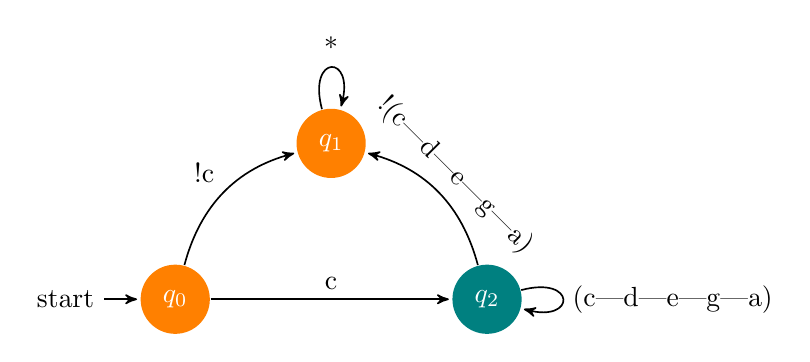
\begin{tikzpicture}[->,>=stealth',shorten >=1pt,auto,node distance=2.8cm,semithick]
  \tikzstyle{every state}=[fill=orange,draw=none,text=white]

  \node[initial,state] (A)                    {$q_0$};
  \node[state]         (B) [above right of=A] {$q_1$};
  \node[state,fill=teal]         (C) [below right of=B] {$q_2$};

  \path (A) edge [bend left]  node {!c} (B)
            edge              node {c} (C)
        (B) edge [loop above] node {*} (B)
        (C) edge [bend right] node [sloped, above] {!(c|d|e|g|a)} (B)
        (C) edge [loop right] node {(c|d|e|g|a)}  (C);
\end{tikzpicture}
\end{center}
\begin{itemize}
\item Memoizing deriv = transition function
\item Memoizing nullable = accept function
\item Simplification = minimization \cite{owens2009regular}
\end{itemize}
\end{frame}

\begin{frame}{Recursive Regular Expressions}

\note{
We can also easily add references for recursion and to help us split our expression into parts,
which we are going to need this to define our Ragas.

For this we need two operators: the definition of a reference and the use of the reference.

The derivative of $@q$ with respect to a is the derivative of whatever q's definition was with respect to a and the same with nullable.
}

\begin{itemize}
\item One extra concept: Reference
\item Two operations
\item Define a reference: $\#myref = (a \cdot b)^{*}$
\item Use a reference: $(@myref\ |\ c)$
\end{itemize}
\begin{center}
\begin{tabular}{l c l}
$\partial_a @q$ & = & $\partial_a \#q$ \\
$\nu(@q)$ & = & $\nu(\#q)$ \\
\end{tabular}
\end{center}
\end{frame}

\section{Ragas - Indian Classical Music}

\note{
Ok, but anyway, sorry for the digression, lets get onto Ragas. 
First I have to thank Ryan Lemmer and Antoine Van Gelder for introducing me to Ragas and
for coming up with the idea to combine Ragas with derivatives.
}

\plain{https://youtu.be/iElMWziZ62A?t=136}

\note{
Here is an example of someone playing a Raga.
See how the player slides his hand up and down the strings.
There are very strict rules that decide what notes he is allowed to play next.
}

\begin{frame}{Ragas}

\note{
Ragas are basically the indian version of western scales.

They are stricter than western scales.

The possible next note is not simply chosen from a set, but rather depends on the current note.

Also notes are labeled a bit differently.

They are labeled relatively to the start note.
So this is simply how they are labeled if you start at c.
}

\begin{itemize}
\item Ragas are indian version of western scales \cite{Raga2011}.
\item Stricter than western scales.
\item Possible next note depends on current note.
\item Notes labeled differently and relative to root note.
\end{itemize}
\begin{center}
\begin{tabular}{l|llllllllllll}
Raga & S & r & R & g & G & m & M & P & d & D & n & N \\
Western & c & c$\sharp$ & d & d$\sharp$ & e & f & f$\sharp$ & g & g$\sharp$ & a & a$\sharp$ & b \\
\end{tabular}
\end{center}
I will skip over microtones and all the other theory, just because its not relevant to this talk.
\end{frame}

\begin{frame}{Example Raga}

\note{
Here is Raag Bhupali a type of Pentatonic scale

Given the current note you must choose the next ascending or descending note.

For example given G you can choose to play P or R next
}

\begin{itemize}
\item Raag Bhupali (a type of Pentatonic scale)
\item Ascent: S R G P D S'
\item Descent: S' D P G R S
\end{itemize}
\begin{itemize}
\item Western Pentatonic scale
\item Ascent: c d e g a c$^{1}$
\item Descent: c$^{1}$ a g e d c
\end{itemize}

Given the current note you must choose the next ascending or descending note.

For example given G (e) you can choose P (g) if you want to ascend or R (d) if you want to descend.
\end{frame}

\plain{\url{http://raag-hindustani.com/22_files/ArohBhupali.mp3}}

\note{Lets listen to this scale}

\plain{Questions?}

\note{
Questions

Is everyone still with us.
After this things start to speed up a little.
It starts to become less of a lesson and more a presentation.
So its good to have this part solid.
}

\begin{frame}{A Grammar for a Raga}

\note{
Ok so here finally we have a raga expressed as a recursive regular expression.

Our first note S is followed by its ascent or descent note and the whole expression is repeated zero or more times.

The ascending note R is ascended by G or descended back to S which is just the empty string, since the termination of the expression results in the end or the repetition of the whole expression which starts with S.

Same goes for the rest.

G is followed by P or R

P is followed by D or G

and D is followed by P or a termination, since it can be followed by S.
}

\begin{itemize}
\item Raag Bhupali (a type of Pentatonic scale)
\item Ascent: S R G P D S'
\item Descent: S' D P G R S
\end{itemize}
\begin{center}
\begin{tabular}{lll}
$\#S$ & = & $(S \cdot ( @R\ |\ @D ))^{*}$ \\
$\#R$ & = & $R \cdot ( @G\ |\ \varepsilon )$ \\
$\#G$ & = & $G \cdot ( @P\ |\ @R )$ \\
$\#P$ & = & $P \cdot ( @D\ |\ @G )$ \\
$\#D$ & = & $D \cdot ( \varepsilon\ |\ @P )$ \\
\end{tabular}
\end{center}
\end{frame}

\plain{Demo}

\note{
Lets see it in action

This program basically does not allow me to play a note that will make the expression go into an emptyset state.

We can even add random input to create a generated piece that satisfies the raga rules.
}

\section{Context Free Grammars}

\note{
I hope you enjoyed that, because now for pudding I have some vegetables.

Don't worry if you don't understand the following part, because it took me quite a while.
I think it is valuable to see some functional concepts applied in a creative way.

Oh and by the way if you are not going to be pendantic then Context free grammars are just another name for recursive regular expressions.
Our example from before was already a context free grammar.
}

\begin{frame}{Left Recursive Raga}

\note{
Here is our expression from before, but just written a bit differently.
We cannot really control how a user uses our expression language, so we have to think of all cases.

The definition of S is either the empty string or it is the S again followed by the expression contained in the original zero or more expression.

You can see how these are equivalent.

Unfortunately this causes infinite recursion for the nullable and derivative function.

We can see that calculating nullable for S requires the calculation of the nullability of S.
}

\begin{center}
\begin{tabular}{lllll}
$\#S$ & {\color{gray}=} & {\color{gray} $(S \cdot ( @R\ |\ @D ))^{*}$} & = & $@S \cdot (S \cdot ( @R\ |\ @D ))\ |\ \varepsilon$ \\
$\#R$ & = & $R \cdot ( @G\ |\ \varepsilon )$ \\
$\#G$ & = & $G \cdot ( @P\ |\ @R )$ \\
$\#P$ & = & $P \cdot ( @D\ |\ @G )$ \\
$\#D$ & = & $D \cdot ( \varepsilon\ |\ @P )$ \\
\end{tabular}
\end{center}


nullable and derivative each have infinite recursion.
$$
\nu(\#S) = (\nu(@S)\ and\ \nu(S \cdot ( @R\ |\ @D )))\ or\  \nu(\varepsilon)
$$
\end{frame}

\begin{frame}{Parsing with Derivatives}

\note{
We are going to solve this problem with 3 functional concepts.

\begin{itemize}
\item laziness
\item memoization
\item least fix points
\end{itemize}

which I like to call the: brake, handbrake and gas respectively.
}

This has been solved using \cite{might2011parsing} functional concepts:
\begin{itemize}
\item laziness - The Brake
\item memoization - The Handbrake
\item least fixed point - The Gas
\end{itemize}
\end{frame}

\begin{frame}[fragile]{Laziness}
\note{
Laziness is when instead of evaluating a function and returning a value,
we defer the evaluation and return a function that will return the value.
Sorry it is kind of hard to demonstrate laziness in haskell, since it is lazy by default.
}

Strict:

\begin{minted}{go}
func eval(params ...) value {
    ...
    return value(...)
}
\end{minted}

Lazy:

\begin{minted}{go}
func lazyEval(params ...) func() value {
    return func() value {
        return eval(params)
    }
}
\end{minted}
\end{frame}

\begin{frame}{Laziness - The Brake}

\note{
Instead of storing the field values of concat, or and zero or more we rather store functions that when called will return the value of the field.

This allows us to avoid any recursion until the value is needed.

I have used the lambda symbol here to represent a thunk or function that will return a value when called with no parameters.

The j is used as shorthand to write concat in a single line.
}

Instead of storing the field values of \textbf{concat}, \textbf{or} and \textbf{zero or more} we rather store functions that when called will return the value of the field.

This allows us to avoid any recursion until the value is needed.

\begin{center}
\begin{tabular}{l c l c l}
$\partial_a (r | s) $ & = & $\partial_a r\ |\  \partial_a s $ 
                      & = & $\lambda(\partial_a r)\ |\  \lambda(\partial_a s) $ \\
$\partial_a (r^{*}) $ & = & $\partial_a r \cdot r^{*}$ 
                      & = & $\lambda(\partial_a r) \cdot r^{*} $ \\
$\partial_a (r \cdot s) $ & = & $\partial_a r \cdot s\ |\  \jmath(r) \cdot \partial_a s $ 
& = &  $\lambda(\lambda(\partial_a r) \cdot s)\ |\  \lambda(\lambda(\jmath(r)) \cdot \lambda(\partial_a s)) $ \\
\end{tabular}
\end{center}

\begin{center}	
\begin{tabular}{l c l r}
$\jmath(r)$ & = & $\epsilon$ & if $\nu(r)$ \\	
 & = & $\emptyset$ & otherwise \\
\end{tabular}	
\end{center}

\begin{center}
\begin{tabular}{l c l}
$\partial_n \#S$ &=& $\lambda(\partial_n(@S \cdot (S \cdot ( @R\ |\ @D ))))\ |\ \lambda(\partial_n \varepsilon)$ \\
\end{tabular}	
\end{center}

\end{frame}

\begin{frame}{Memoization - The Handbrake}
\note{
Eventually nullability is going to be called and this won't be stopped by laziness alone.

The point of these equations are that we still need the nullability of the derivative of S to calculate the nullability of the derivative of S.

Memoizing helps to close the loop.

It stops the recursive execution of the derivative by only calculating the derivative once and returning the same lazy function for following executions.x
}

Eventually nullable is going to be called.
\begin{center}
\begin{tabular}{lll}
$\nu(\partial_n \#S)$ & = & $\nu(\lambda(\partial_n(@S \cdot (S \cdot ( @R\ |\ @D ))))\ |\ \lambda(\partial_n \varepsilon))$\\
& = & $\nu(\lambda(\partial_n(@S \cdot (S \cdot ( @R\ |\ @D )))))\ |\ \nu(\lambda(\partial_n \varepsilon))$\\
\end{tabular}
\end{center}
Which will result in the execution of a lazy derivative function.
\begin{center}
\begin{tabular}{lll}
$\lambda(\partial_n (@S \cdot (S \cdot ( @R\ |\ @D )))) $ & = &
$\partial_n (@S \cdot (S \cdot ( @R\ |\ @D ))) $ \\
&=&$\lambda(\lambda(\partial_n @S) \cdot \lambda((S \cdot ( @R\ |\ @D ))))\ |$\\
&& $\lambda(\lambda(\jmath(@S)) \cdot \lambda(\partial_n (S \cdot ( @R\ |\ @D )))) $ \\
$\lambda(\partial_n @S)$ &=& $\partial_n @S$ \\
\end{tabular}
\end{center}
Which can result in infinite recursion.
\begin{center}
\begin{tabular}{lll}
$\partial_n @S$ &=& $\partial_n \#S$ \\
\end{tabular}
\end{center}

Memoizing helps by closing the loop.

\begin{center}
\begin{tabular}{lll}
$\partial_n @S$ &=& $\lambda(\partial_n(@S \cdot (S \cdot ( @R\ |\ @D ))))\ |\ \lambda(\partial_n \varepsilon)$ \\
\end{tabular}
\end{center}

\end{frame}

\begin{frame}[fragile]{Memoization}

\note{
Memoizing a function is when you cache the results for given inputs and so only calculate the value once.
Just like caching it is typically a great way to optimize your code.
So in this case, we are using it to close a loop, but it is not enough.
We need another tool.
}

\begin{minted}{go}
func memoize(eval func(a) b) func(a) b {
    mem := make(map[a]b)
    return func(input a) b {
        if output, ok := mem[input]; ok {
            return output
        }
        output := eval(a)
        mem[input] = output
        return output
    }
}
\end{minted}

\end{frame}

\begin{frame}[fragile]{Least Fixed Point}
\note{
A fixed point of a function is when the function result equals the input.
For example: x squared has two fix points, one and zero.
The least fixed point would be the zero, since it is smaller than one.
}
\begin{center}

$$f(x) = x^2$$
$$f(0) = 0^2$$
$$f(1) = 1^2$$

fixed points = $\{0, 1\}$

least fixed point = $0$

\end{center}
\end{frame}

\begin{frame}[fragile]{Least Fixed Point of Derivative}
\note{
What fixed points do we have for the derivative function?
The derivative of the empty set is always the empty set,
but the derivative of a star given a is also a star.
I would think that the empty set is the least fixed point, given that it is the simplest expression.
}
\begin{center}

$$\partial_a r\ = r\ $$
$$\partial_a \emptyset\ = \emptyset\ $$
$$\partial_a a^{*} = a^{*}$$

fixed points = $\{\emptyset, a^{*}\}$

least fixed point = $\emptyset$

\end{center}
\end{frame}

\begin{frame}{Least Fixed Point - The Gas}

\note{
Eventually nullable still needs to return a true or a false.

We can use our least fixed point, to return a derivative of empty set when nullable revisits the same expression.
}

Nullable is relentless:

\begin{center}
\begin{tabular}{lll}
$\nu(\lambda(\partial_n \#S))$ &=& $\ldots$\\
$\nu(\lambda(\partial_n(@S \cdot (S \cdot ( @R\ |\ @D )))))\ |\ \nu(\lambda(\partial_n \varepsilon))$ &=& $\ldots$ \\
$\nu(\lambda(\lambda(\partial_n @S) \cdot \lambda(\ldots)))$& = & $\ldots$ \\
$\nu(\lambda(\partial_n @S))$   &=& $\nu$({\color{mLightGreen} fix}) \\
                                &=& $\nu$({\color{mLightGreen} $\emptyset$}) \\
                                &=& {\color{mLightGreen} false} \\
$\nu(\lambda(\lambda(\partial_n @S) \cdot \lambda(\ldots)))$& = & {\color{mLightGreen} false} \& false \\
$\nu(\lambda(\partial_n(@S \cdot (S \cdot ( @R\ |\ @D )))))\ |\ \nu(\lambda(\partial_n \varepsilon))$ &=& {\color{mLightGreen} false} | false\\
$\nu(\lambda(\partial_n \#S))$ &=& {\color{mLightGreen} false} \\
\end{tabular}
\end{center}
\end{frame}

\plain{\url{http://awalterschulze.github.io/ragax/}}

\note{
Here we see both versions of the grammars and how they both validate the same strings.
}

\begin{frame}{Yacc is Dead}

\note{
Now we have a fully generalized Context Free Grammar validator.

Yacc, Antlr, Flex, Bison, etc.  definitely still performs better, especially in worst case.

But derivatives:

\begin{itemize}
\item are a lot easier to implement and understand than LR(1), LL(1), LALR parsers
\item are implemented using only functional techniques
\item can validate the full set of Context Free Grammars, not just a subset.
\end{itemize}

}

Yacc, Antlr, Flex, Bison, etc.  perform better.

But derivatives:
\begin{itemize}
\item more intuitive than LR(1), LL(1), LALR parsers;
\item only use functional techniques;
\item recognize generalized Context Free Grammars, not just a subset.
\end{itemize}
\end{frame}

\section{Trees}

\note{Finally lets quickly brush over trees}

\begin{frame}{Relaxing}

\note{
The expressions recognized by derivatives can be polymorphic.
They don't need to only apply to characters.
They can rather refer to XML Nodes and this is how the RelaxNGs implementation and specification is done.
RELAX NG is a schema language for XML, like XSchema and DTD.
Relaxing also introduces some extra operators: Not, Compliment, Interleave and Optional.

With interleave the derivative can take the derivative of any one of the interleaving patterns.
The other pattern needs to keep its original form.
Nullability is easy.

Not, like all the logical operators just passes its problem down.

And optional is just syntactic sugar.
}

http://relaxng.org/ \cite{Relaxng2014} - RELAX NG is a schema language for XML, like XSchema and DTD.

Derivatives used for Implementation and Specification.

Polymorphic Regular Expressions: Characters $=>$ XMLNodes.

New Operators:
\begin{center}
\begin{tabular}{l c l}
$\partial_a (r\ \&\&\ s) $ & = & $(\partial_a r\ \&\&\ s)\ |\ (\partial_a s\ \&\&\ r)$ \\
$\nu(r\ \&\&\ s)$ & = & $\nu(r)$ and $\nu(s)$ \\
$\emptyset\ \&\&\ r$ & $\approx$ & $\emptyset$ \\
$\varepsilon\ \&\&\ r$ & $\approx$ & $r$ \\
\\
$\partial_a !(r) $ & = & $!(\partial_a r)$ \\
$\nu(!(r))$ & = & not($\nu(r)$)\\
\\
$(r)?$ & $\approx$ & $r\ |\ \varepsilon$ \\
\end{tabular}
\end{center}
\end{frame}

\begin{frame}[fragile]{TreeNode}

\note{
The "hard" part is defining deriative function for the XML or Tree node operator.
Here is an implementation in Haskell.

The TreeNode pattern has a name expression and a child expression.
To keep it basic I have made the name expression just a plain string.

The Node has a label string and a list of child nodes.
If the name expression equals the label string we have to take the derivative of the children.
Otherwise we return the empty set just like with a character.

If the result of taking the derivative of the children is nullable we return the empty pattern else we return the empty set.
Nullability of a treenode is always false, just like a character.
}

\begin{haskellcode}
deriv :: Expr -> Tree -> Expr
deriv (TreeNode nameExpr childExpr) 
      (Node name children) = 
  if nameExpr == name then
     let childDeriv = foldl deriv childExpr children
     in if nullable childDeriv
        then Empty
        else EmptySet
  else EmptySet
    
nullable (TreeNode _ _) = False
\end{haskellcode}
\end{frame}

\plain{\url{https://youtu.be/SvjSP2xYZm8} \url{katydid.github.io}}

\begin{frame}{Katydid: Relapse}

\note{
Finally the thing I am actually working on.
Katydid is a tree toolkit, which includes Relapse: a validation language based on relaxing.

I use derivatives and memoization to build a visual pushdown automata.
This allows me to do matching with zero memory allocations once the automata has been compiled.

I support: Json, Protobuf, XML and reflected structures, but its easy to add your own parser.
I currently have implementations in Go and Haskell.

I also added some new operators: And, Contains and ZAny.
Zany is just zero or more of anything, like .* in a regular expression.
Which is just syntatic sugar for the compliment of the emptyset.
And, again like all logical operators, just passes its problem down.
Contains is just syntatic sugar for an expression surrounded by concatenated zanys.
}

Relapse: Tree Validation Language.

JSON, Protobufs, Reflected Go Structures and XML

Go, Haskell + Cross language testsuite

New Operators:
\begin{center}
\begin{tabular}{l c l}
$\partial_a (r\ \&\ s) $ & = & $(\partial_a r\ \&\ \partial_a s)$ \\
$\nu(r\ \&\ s)$ & = & $\nu(r)$ and $\nu(s)$ \\
$\emptyset\ \&\ r$ & $\approx$ & $\emptyset$ \\
$r\ \&\ r$ & $\approx$ & $r$ \\
\\
$*$ & $\approx$ & $!(\emptyset)$ \\
\\
$.r$ & $\approx$ & $* \cdot r \cdot *$ \\
\end{tabular}
\end{center}

\url{https://github.com/katydid/katydid-haskell}
\end{frame}

\plain{\url{http://katydid.github.io/play/} \url{http://katydid.github.io/tour/}}

\note{
I can now show you the playground.

And I also have a tour.
}

\begin{frame}{References}

\note{Thank you for listening.}

\bibliography{ragax}
\bibliographystyle{abbrv}

\end{frame}

\end{document}
